\documentclass[9pt,handout]{beamer}
\usepackage{pgfpages}
\pgfpagesuselayout{2 on 1}[a4paper,border shrink=12mm]

\usepackage[latin1]{inputenc}
\usepackage[english]{babel}
\usepackage{graphics}
%\usepackage{includegraphix}
\usepackage{hyperref}
\usepackage{units}
%\usepackage{listings}
%\lstset{%
%  language=C++,
%  numbers=left, 
%  numberstyle=\tiny,
%  frame=single
%}
%
\usepackage{amsmath}
\usepackage{amsfonts}
\usepackage{amssymb}

\usepackage{color}

\usepackage{amsmath}
\usepackage{tikz}
\usetikzlibrary{calc}
\usetikzlibrary{shapes}

\useoutertheme{infolines}
\usetheme[]{default}
\setbeamertemplate{navigation symbols}{}
\setbeamertemplate{bibliography item}[text]
\setbeamertemplate{blocks}[rounded][shadow=true]
\setbeamertemplate{caption}[numbered]
\definecolor{somegrey}{RGB}{240,240,240}

\setbeamercolor{block title}{bg=black!60!white,fg=white}
\setbeamercolor{block title alerted}{use=alerted text,fg=blue!40!white,bg=black!60!white}
\setbeamercolor{block title example}{bg=black!20!white}

%\addfootbox{bg=grey,fg=black}{\quad \insertshortauthor \hspace{.4\textwidth} \insertshortinstitute \hspace{.4\textwidth} \insertpagenumber}

\begin{document}


\pgfdeclareimage[height=1.5cm]{ATLASlogo}{img/AN_atlaslogo}
\pgfdeclareimage[height=1.5cm]{FSPlogo}{img/FSPAtlas_logo}
\pgfdeclareimage[height=.8cm]{TUDlogo}{img/logo_schwarz}
\titlegraphic{ \hspace{2cm} \pgfuseimage{TUDlogo} \hfill \pgfuseimage{ATLASlogo} \hfill \pgfuseimage{FSPlogo}\hspace{2cm} }

\title[Class Design Principles]{ Class Design Principles in Object-Oriented Programming }
%\subtitle{- A  -}
\author[P. Steinbach]{Wolfgang F. Mader, \textbf{Peter Steinbach}}
\date{March 10th, 2011}

\institute[IKTP]{Institute for Nuclear and Particle Physics, TU Dresden}



\begin{frame}
  \vfill
  \begin{center}
    \begin{block}{From the Gaudi User Guide, \cite{gug}}
      \begin{quotation}
        A priori, we see no reason why moving to a language which supports the idea of objects, such as \texttt{C++}, should change the way we think of doing physics analysis.
      \end{quotation}
    \end{block}
    \huge
    Why Use Object-Oriented Programming in the First Place?
  \end{center}

  \vfill
\end{frame}

\maketitle

\begin{frame}
\frametitle{Outline}
\tableofcontents
\end{frame}

\section[Why OOP?]{Why Object-Oriented Programming?}
\subsection[ProceduralVsOO]{Procedural versus OO Programming}
\begin{frame}
\frametitle{Procedural vs. OO Programming, from \cite{Stefan}}
\begin{columns}[c]
  \begin{column}{.49\textwidth}

      \begin{block}{the procedural paradigm}
        \begin{center}
        \resizebox{.85\textwidth}{!}{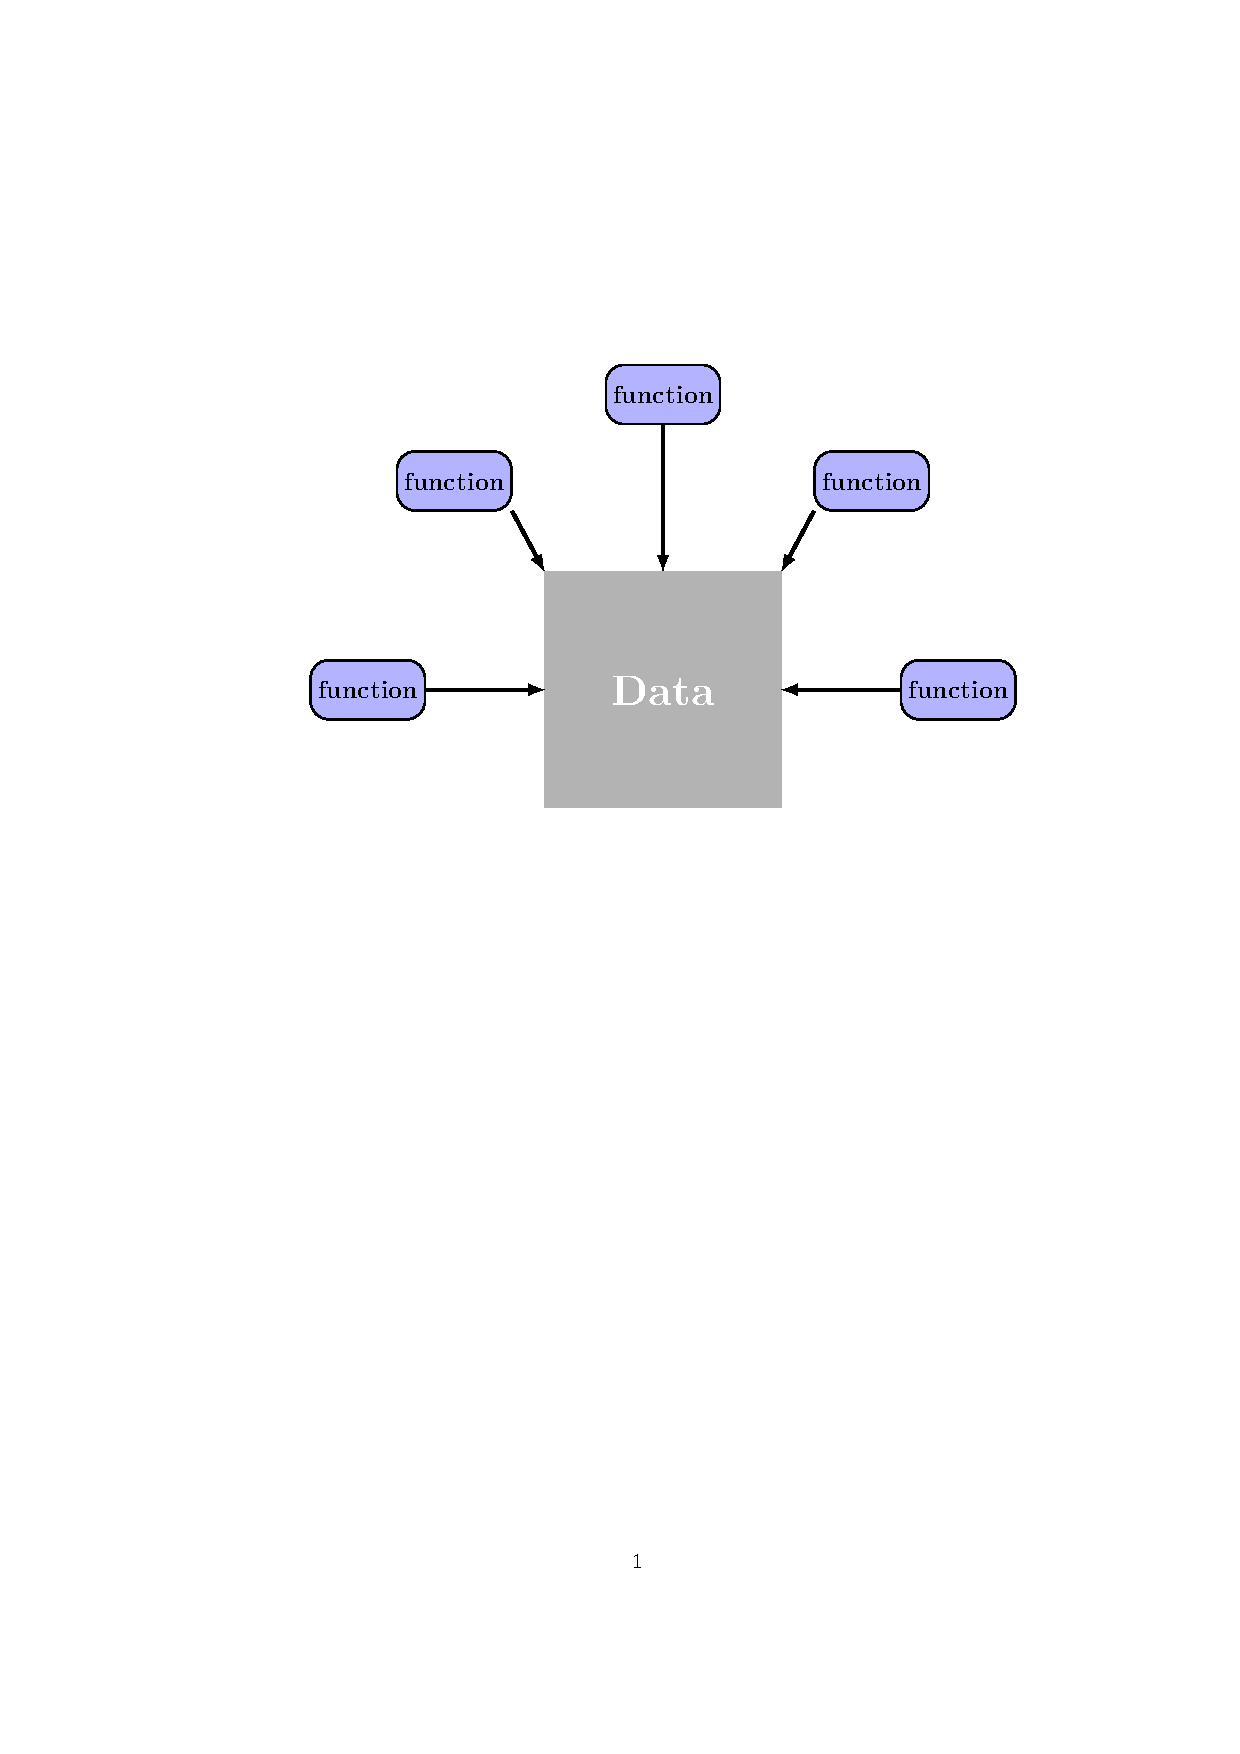
\includegraphics{img/procedural}}
      \end{center}
      \end{block}
   
  \end{column}
\hfill
\pause
  \begin{column}{.49\textwidth}

      \begin{block}{the oo paradigm}
        \begin{center}
        \resizebox{1.\textwidth}{!}{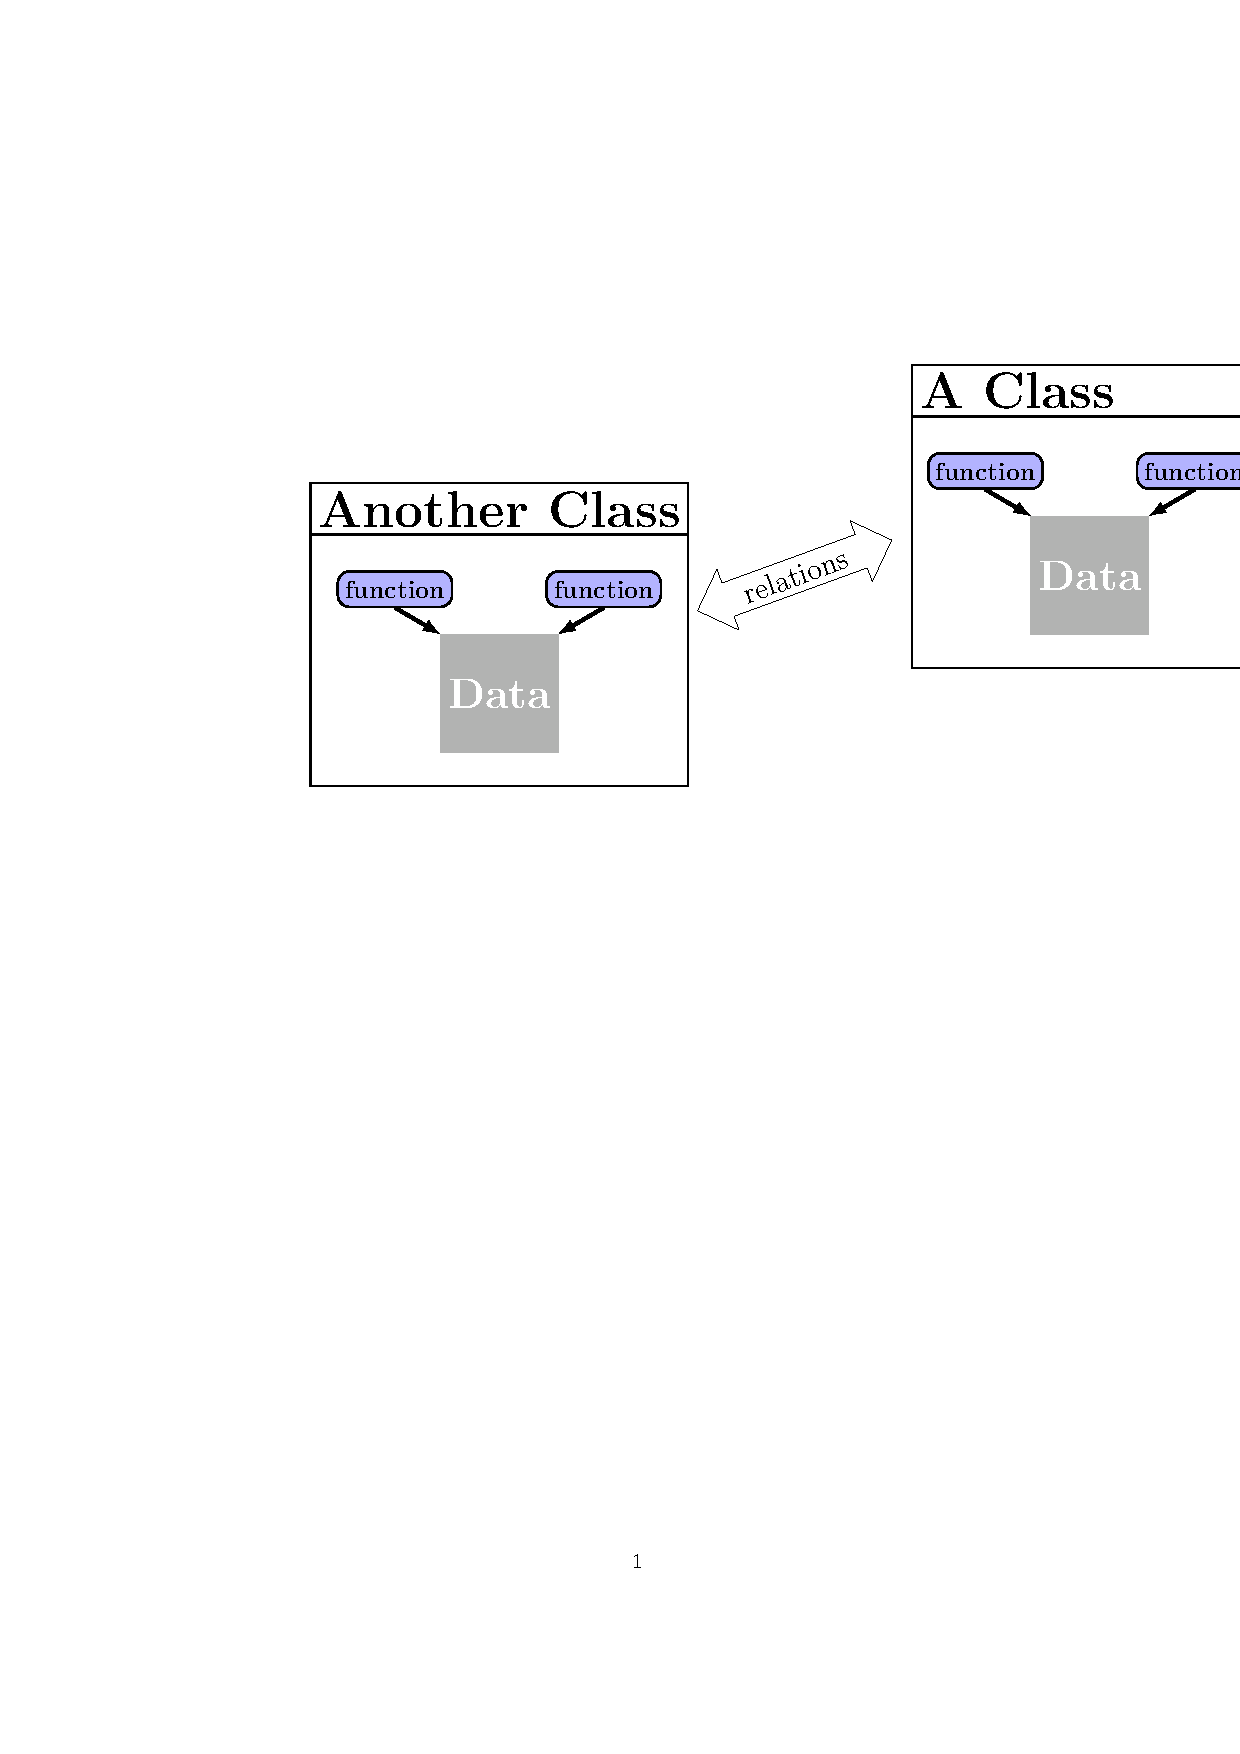
\includegraphics{img/oop}}
        \end{center}
      \end{block}
      
  \end{column}

\end{columns}
\vfill
\begin{columns}[c]
  \begin{column}{.49\textwidth}
    \begin{center}
      \huge
      \alert{Top-Down}
  
    \end{center}
  \end{column}
  \begin{column}{.49\textwidth}
    \begin{center}
      \huge
      \alert{Bottom-Up}
    \end{center}
  \end{column}
\end{columns}
\end{frame}

\subsection[Hep Software]{HEP Programming}
\begin{frame}
\frametitle{Hep Software Sizes}
\begin{block}{A History of Code}
  \begin{center}
    \Large
    \begin{tabular}[h]{l|p{5cm}}
      & lines of code / $\unit[1]{loc}$ \\[12pt]
      JADE & $o(10-100)k$\\[12pt]
      OPAL & $o(100)k$\\[12pt]
      ATLAS & $o(1)M$
    \end{tabular}
  \end{center}
\end{block}
\vfill
\begin{itemize}
\item<2-> experiments size and complexity increases 
\item<3-> experiments analysis software size and complexity increases
\item<4-> \Large \alert{We need tools that deal with this complexity!}
\end{itemize}

\end{frame}

\subsection[OOP in HEP]{Programming Paradigms in HEP}
\begin{frame}
\frametitle{Programming Paradigms in HEP}
\normalsize
\begin{block}{physics is about ...}
  \begin{itemize}
  \item \alert<4->{modelling nature}
  \item objects interact according to laws of nature
    \begin{itemize}
    \item fields, particles, atoms, molecules, solid states, liquids
    \end{itemize}
  \end{itemize}
\end{block}
\vfill
\pause
\begin{block}{object-oriented programming is about ...}
  \begin{itemize}
  \item \alert<4->{objects and interactions}
    \begin{itemize}
    \item a way of thinking about software well adapted to
      physics
    \end{itemize}

  \end{itemize}
\end{block}
\vfill
\pause
\begin{block}{object-oriented analysis and design ...}
  \begin{itemize}
  \item is a software engineering practice
  \item \alert<4->{manages large projects professionally}
  \end{itemize}
\end{block}
\end{frame}

\section{Orthogonality}
\begin{frame}
  \frametitle{Orthogonality}
  \begin{definition}
    A \textbf{Responsibility} of a class is defined as \emph{a reason for the class to change}.
  \end{definition}
  %Modem, TSystem examples
  \vfill
  \pause
  \begin{exampleblock}{Exercise 1}
    \begin{center}
      \Large
      How many responsibilities do classes a) and b) have?
    \end{center}
  \end{exampleblock}
\pause
  \vfill
  \begin{definition}
    \textbf{Orthogonality}(\cite{PP}) of a system of classes can be defined as the degree of how many classes have independent or non-overlapping \emph{responsibilities}.
  \end{definition}

\end{frame}


\begin{frame}
  \frametitle{Single-Responsibility Principle}
  \begin{theorem}[from \cite{Agile}]
    A class should only have \textbf{one} reason to change, i.e. try to create systems with high orthogonality.
  \end{theorem}
\vfill
\pause
\begin{exampleblock}{Looking back at Exercise 1 a)}
  \begin{columns}[t]
    \begin{column}{.48\textwidth}
       \begin{block}{before}

          \begin{center}
               \resizebox{.65\textwidth}{!}{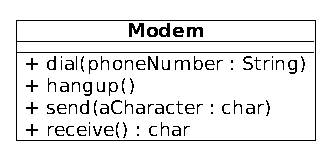
\includegraphics{uml/modem}}
          \end{center}
      %   
       \end{block}
 %     
    \end{column}
\hfill
    \begin{column}{.48\textwidth}
       \begin{block}{after}
       \begin{center}
         \resizebox{.85\textwidth}{!}{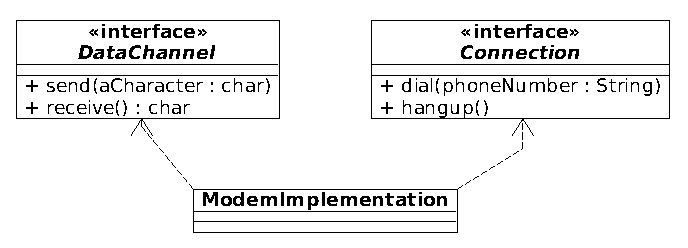
\includegraphics{uml/modemImplementation}}
       \end{center}
      \end{block}
    \end{column}
  \end{columns}
\end{exampleblock}
\end{frame}

\section{Open-Closed Principle}
\begin{frame}
  \frametitle{The \secname}
  \begin{theorem}[from \cite{Agile}]
    Software Entities (classes, modules, functions, etc) should be open for extenstion, but closed for modification.
  \end{theorem}
\vfill
\pause
  \begin{columns}[t]
    \begin{column}{.48\textwidth}
       \begin{block}{Open}
         \begin{itemize}
         \item<3-> the \textbf{behavior} of an entity can be extended
         \item<3-> as requirements of a system change (that's a fact!), the entities behavior can be \textbf{extended or modified} to satisfy these changes
         \end{itemize}
       \end{block}
 %     
    \end{column}
\hfill
    \begin{column}{.48\textwidth}
       \begin{block}{Closed}
         \begin{itemize}
         \item<4-> extension of behavior does \textbf{NOT} result in changing the source code 
         \item<4-> the binary executable version of a given entity remains \textbf{untouched}
         \end{itemize}
      \end{block}
    \end{column}
  \end{columns}

\uncover<5->{
\begin{exampleblock}{Exercise 2}
  \begin{center}
    The above is way too complicated for one slide! Let's have a look
    at \textbf{Exercise 2}!
  \end{center}

\end{exampleblock}
}
\end{frame}


\begin{frame}[fragile]
  \frametitle{Reviewed: \secname}
  \begin{block}{The Square/Circle Problem}
    \begin{itemize}
    \item \emph{rigid}: adding triangle requires \texttt{Shape, Square, Circle, DrawAllShapes} to be recompiled and redeployed
    \item \emph{fragile}: \texttt{switch/case} will be required by all client classes that use \texttt{Shape}s
    \item \emph{immobile}: reusing \texttt{DrawAllShapes} is impossible without including \texttt{Shape, Square, Circle} as well
    \end{itemize}
  \end{block}
\pause
\begin{block}{Solution: Using Abstraction}
    
    \begin{columns}[t]
      \begin{column}{.45\textwidth}
        \small
        \begin{semiverbatim}
struct Shape \{ 
  virtual void Draw() const = 0; 
\}

struct Square \{ 
  virtual void Draw() const; 
\}
        \end{semiverbatim}
      \end{column}
      \begin{column}{.45\textwidth}
        \scriptsize
        \begin{semiverbatim}
void DrawAllShapes(
  const std::vector<Shape*>& list) \{

  std::vector<Shape*>::const_iterator itr; 

  for(itr=list.begin();itr!=list.end(); ++itr) 
  \{ 
    itr->Draw(); 
  \}

\}
        \end{semiverbatim}
      \end{column}

    \end{columns}

  \end{block}



\end{frame}

\begin{frame}
  \frametitle{Summary: The \secname}
\begin{block}{But hold on ...}
  \begin{itemize}
  \item<1-> did the abstraction from above close \texttt{DrawAllShapes} against all changes?
    \begin{itemize}
    \item \textbf{No}, there is no model of abstraction that is natural to all
      contexts!
    \item closure can never be complete, only strategic
    \end{itemize}
  \item<2-> how to deal with possible changes?
    \begin{enumerate}
    \item derive possible changes from software requirements
    \item implement necessary abstractions
    \item wait!
    \end{enumerate}
  \end{itemize}
\end{block}
\vfill
\pause
\begin{block}{To Summarize}<3->
  \begin{itemize}
  \item conforming to the open-closed principle yields greatest benefits of OOP (flexibility, reusability, maintainability)
  \item apply abstraction to parts of software that exhibit frequent change
  \item \alert<3->{Resisting premature abstraction is as important as abstraction itself.}
  \end{itemize}
\end{block}
\end{frame}

\section{Liskov Substitution Principle}
\begin{frame}
  \frametitle{The \secname}
  \begin{theorem}[paraphrased from \cite{Liskov}]
    Subtypes must be substitutable for their base types.
  \end{theorem}
\pause
\vfill
\begin{exampleblock}{Exercise 3}
  \begin{center}
    Try to answer question 3 a) and b) !
  \end{center}
\end{exampleblock}
\end{frame}

\begin{frame}
  \frametitle{Review \& Summary: The \secname}
  \begin{block}{Observations from Exercise 3}
    \begin{itemize}
    \item<2-> Violations of {\secname} result in Run-Time Type Information to be used
      \begin{itemize}
      \item violates the Open-Closed Principle
      \end{itemize}
    \item<3-> an (inheritance) model can never be validated in isolation 
      \begin{itemize}
      \item but rather with its use (users) in mind
      \item \texttt{Is-A} relationship within inheritance refers to \textbf{behavior} that can be \textbf{assumed} or that \textbf{clients depend upon}.
      \end{itemize}
    \item<4-> how to ensure/enforce \secname?
      \begin{itemize}
      \item Design-by-Contract 
      \item in C++: only by assertions or Unit Tests
      \end{itemize}
    \end{itemize}
  \end{block}
\pause
\vfill
\begin{block}{Summary}<5->
  \begin{itemize}
  \item this principle ensures: maintainability, reusability, robustness
  \item {\secname} enables the Open-Closed Principle
  \item the contract of a base type has to be well understood, if not even enforced by the code
  \end{itemize}
\end{block}
\end{frame}

\section{Dependency-Inversion Principle}
\begin{frame}
  \frametitle{The \secname}
  \begin{theorem}[from \cite{Agile}]
    \begin{enumerate}
    \item High level modules \textbf{should not depend} upon low
      level modules. Both should depend upon abstractions.
    \item Abstractions \textbf{should not depend} upon details. details
      should depend upon abstractions.
    \end{enumerate}
  \end{theorem}
\pause
\vfill
\begin{exampleblock}{Exercise 4}
  \begin{center}
    Please complete 4 a)!
  \end{center}
\end{exampleblock}
\end{frame}

\begin{frame}
  \frametitle{Observations: The \secname}
\begin{exampleblock}{Exercise 4 continued}
  \begin{enumerate}
  \item The vendor of \texttt{Lamp} changes it's definition. All methods containing \texttt{Turn} are renamed to \texttt{Ramp}! Face your design with that!
    \pause
  \item Look at \texttt{Button}: Can it be reused for classes of type \texttt{Signal}?
  \end{enumerate}
\end{exampleblock}
\pause
\begin{exampleblock}{Exercise 4: A Solution}
  \begin{columns}[t]

    \begin{column}{.45\textwidth}
       \begin{block}{Naive Ansatz}

          \begin{center}
               \resizebox{.95\textwidth}{!}{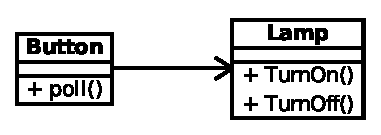
\includegraphics{uml/ButtonNaive}}
          \end{center}
      %   
       \end{block}
 %     
    \end{column}

    \begin{column}{.45\textwidth}
       \begin{block}{Inverted Dependency}
       \begin{center}
         \resizebox{.85\textwidth}{!}{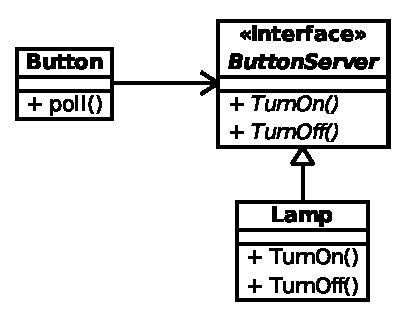
\includegraphics{uml/ButtonInverse}}
       \end{center}
      \end{block}
    \end{column}

  \end{columns}
  
\end{exampleblock}
\end{frame}

\begin{frame}[fragile]
  \frametitle{Review: The \secname}
\vfill
\begin{block}{Dynamic and Static Polymorphism}
\small
in C++, both can help to invert dependencies\\
\begin{columns}[t]

    \begin{column}{.45\textwidth}
       \begin{block}{Dynamic Polymorphism through Abstract Interfaces}

          \begin{center}
               \resizebox{!}{.4\textheight}{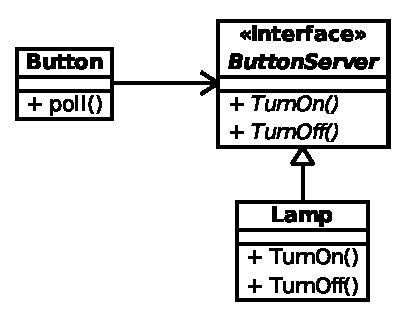
\includegraphics{uml/ButtonInverse}}
          \end{center}
      %   
       \end{block}
 %     
    \end{column}
\pause
    \begin{column}{.45\textwidth}
       \begin{block}{Static Polymorphism through template classes}

          \begin{center}
            \scriptsize
              \begin{semiverbatim}
template <class TurnableObject>
class Button \{

TurnableObject* itsTurnable;

public:
  Button(TurnableObject* _object = 0 ): 
    itsTurnable(_object)
    \{\};

  void poll() \{
    if(/*some condition*/)
      itsTurnable.TurnOn();
    \}
\};
              \end{semiverbatim}
%               % \resizebox{!}{.4\textheight}{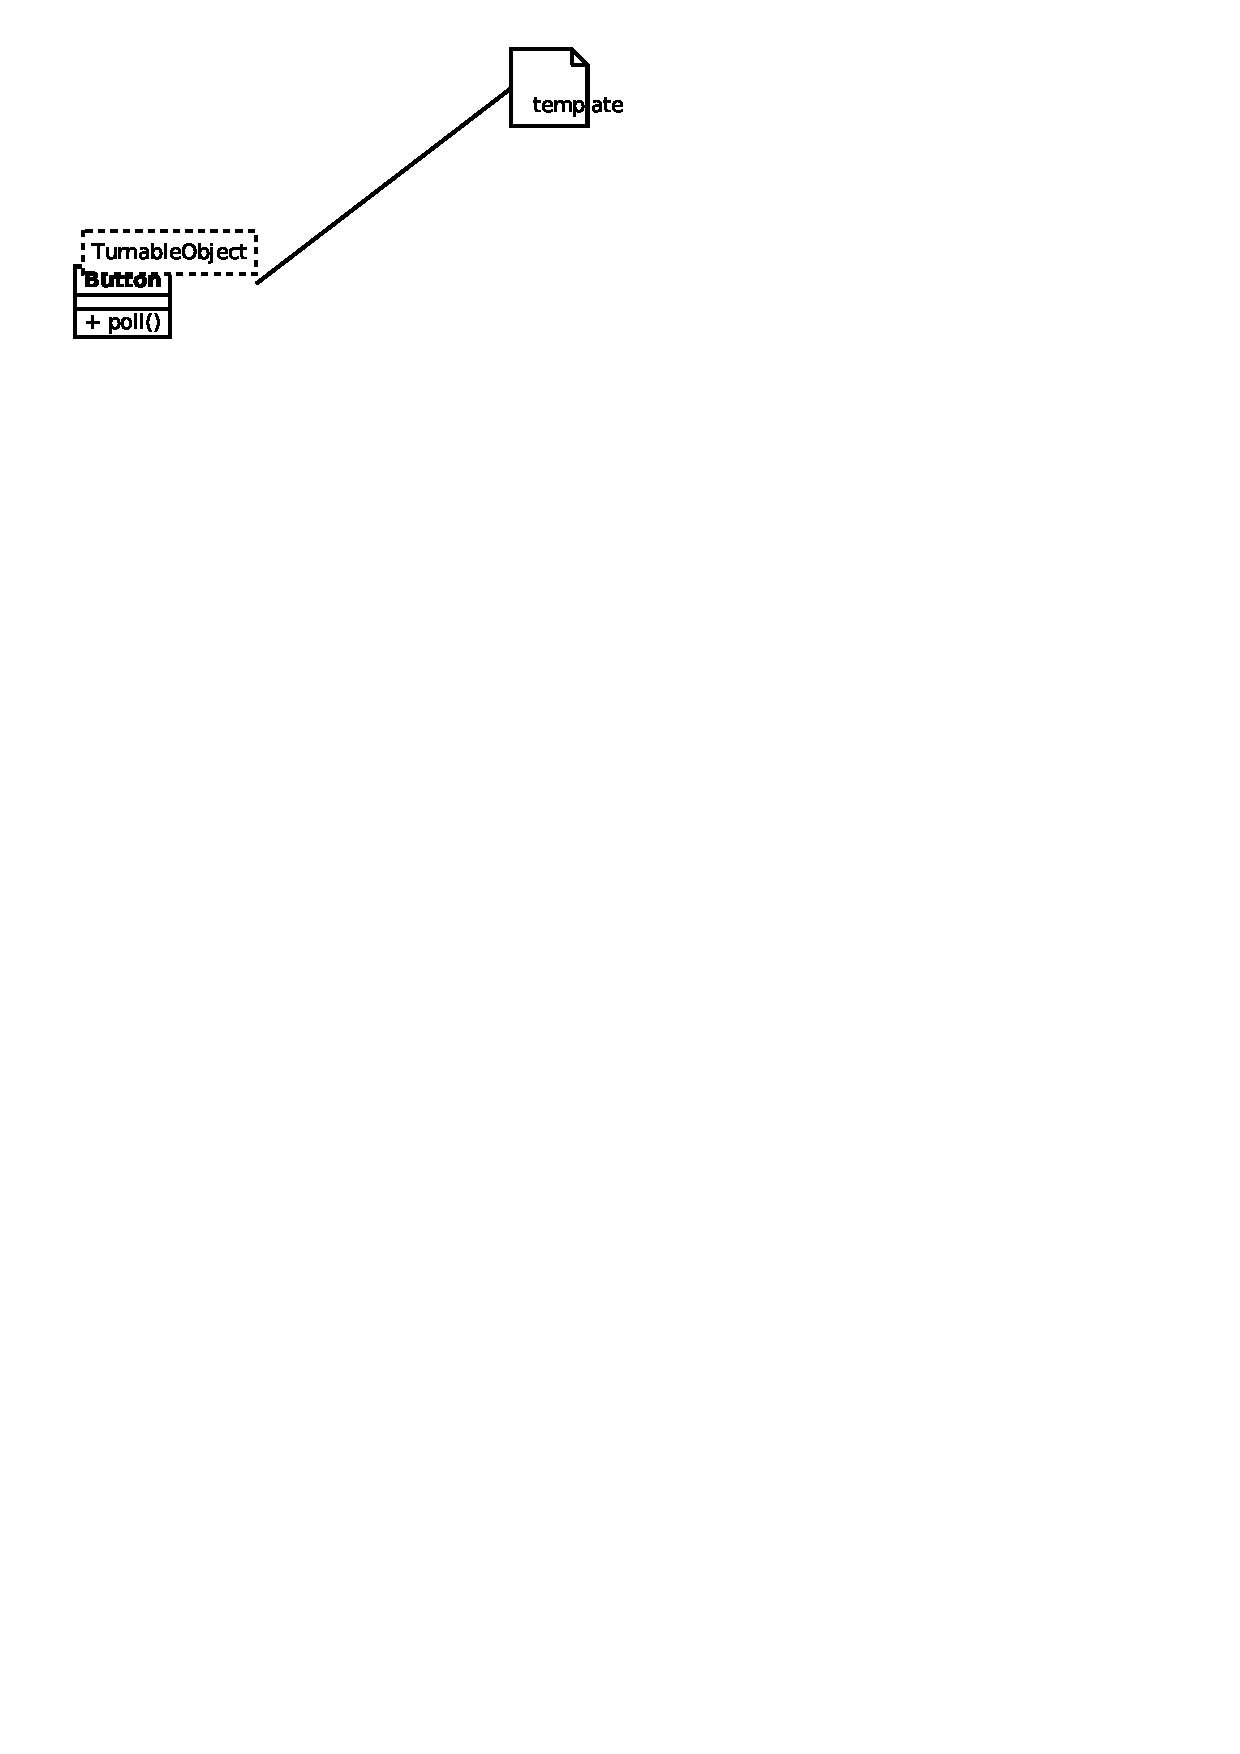
\includegraphics{uml/ButtonTemplate}}
          \end{center}
        \normalsize
        \begin{itemize}
        \item compile-time polymorphism
        \item design-by-policy, see \cite{alexandrescu}
        \end{itemize}
      \end{block}
    \end{column}

  \end{columns}
  \end{block}
\end{frame}

\begin{frame}
  \frametitle{Summary: The \secname}
\begin{block}{Summary}
  \begin{itemize}
  \item dependency of policies on details is natural to procedural design
  \item inversion of dependencies is hallmark of (good) object-oriented design
  \item {\secname} is at the heart of reusable frameworks (no matter what size)
  \item enables the Open-Closed Principle
  \end{itemize}
\end{block}
\end{frame}

\section{Summary}
\begin{frame}
  \frametitle{\secname}
  \begin{block}{What is left to say ...}
    did not cover:
    \begin{itemize}
    \item module design principles
    \item clean code principles
    \item useful coding conventions
    \end{itemize}
  \end{block}
\vfill
\pause
  \begin{block}{What I tried to say ...}
    \begin{itemize}
    \item although having a slow learning curve, OOP can help do highly-sophisticated physics analysis
    \item learning OO Class Design prevents sleepless nights of debugging or copy-and-past'ing
    \item Coding may not be our profession, but we do it everyday anyhow, so we better know our craft!
    \end{itemize}
  \end{block}
\end{frame}

\section{References}
\scriptsize
\begin{frame}
  \frametitle{References}
  \bibliographystyle{plain} 
  \bibliography{Mar10.ClassDesign}
\end{frame}
\end{document}




